% =====================================================================================
% fig_prototypes.tex: what the prototypes are (Q4; Notion E11 qualitative figures).
%
% What the experiment tests: after push, each node prototype is a real training node; its
%   cared bits are trunk units, each decodable (at least for L0) into a rule over the
%   node's neighbourhood. A prototype card shows the prototype's source node in its graph,
%   its cared bits as readable conditions, and the test nodes that match it best.
% Plot: one card per informative prototype (cited by the head, >= 1 cared bit), for
%   Mutagenicity (expected: nitro / amine, substituted aromatic carbon, sulfonyl/F, as
%   found on fold 5 of the hand-tuned NMP) and BAMultiShapes (expected: motif nodes).
%   Each card: the molecule / graph with matched nodes highlighted and the ground-truth
%   region shaded; the cared bits as "L0u41: N with 2 O neighbours"-style conditions;
%   mismatch counts of the match ("<= 3 mismatches") rather than "matches".
% What it shows: that prototypes correspond to recognisable substructures and coincide
%   with the ground truth where one exists (quantified by GT precision in
%   table_interp.tex).
% What it does not show: that every prototype is meaningful (selection bias: say how the
%   cards were picked and show all cited prototypes in the appendix); that the head uses
%   them correctly.
% Data: explain_proto.py / utils/viz_proto.py (plot_proto.py --inside N), or an explorer
%   export; final NMP+QAT fold chosen by a stated rule (same fold as fig_agreement).
% FIXED: viz_proto "no node matches Pk" label (202b569, now mismatch counts); two-band
%   head literals were labelled "always true" (a771fe3 multi-band labels, fca168a exact
%   intervals).
% GENERATED BY: python plot_paper.py prototypes   (sources: configs/paper_figures.yaml, code:
%   utils/paper_figures.py, branch feat/paper-figures). "preliminary: true" in the config
%   stamps PRELIMINARY on the figure; set it to false only when every source is final.
% STATUS: PRELIMINARY version drawn 2026-10-21. Prototypes are ranked by EVIDENCE citations (3c0a4f3: constant head literals are a bias and cite nothing); the first version ranked by all citations and showed constant "always true" prototypes. The cards are also too text-heavy for a paper page: plan a compact version (graph + 2-3 decoded L0 conditions).
% TODO:
%   [x] fix head literal captions; cards ranked by evidence -> fig_prototypes_<ds>.pdf.
%   [ ] appendix: all cited prototypes of that fold.
% =====================================================================================
\begin{figure*}[t]
  \centering
  \IfFileExists{figures/fig_prototypes_Mutagenicity.pdf}{%
    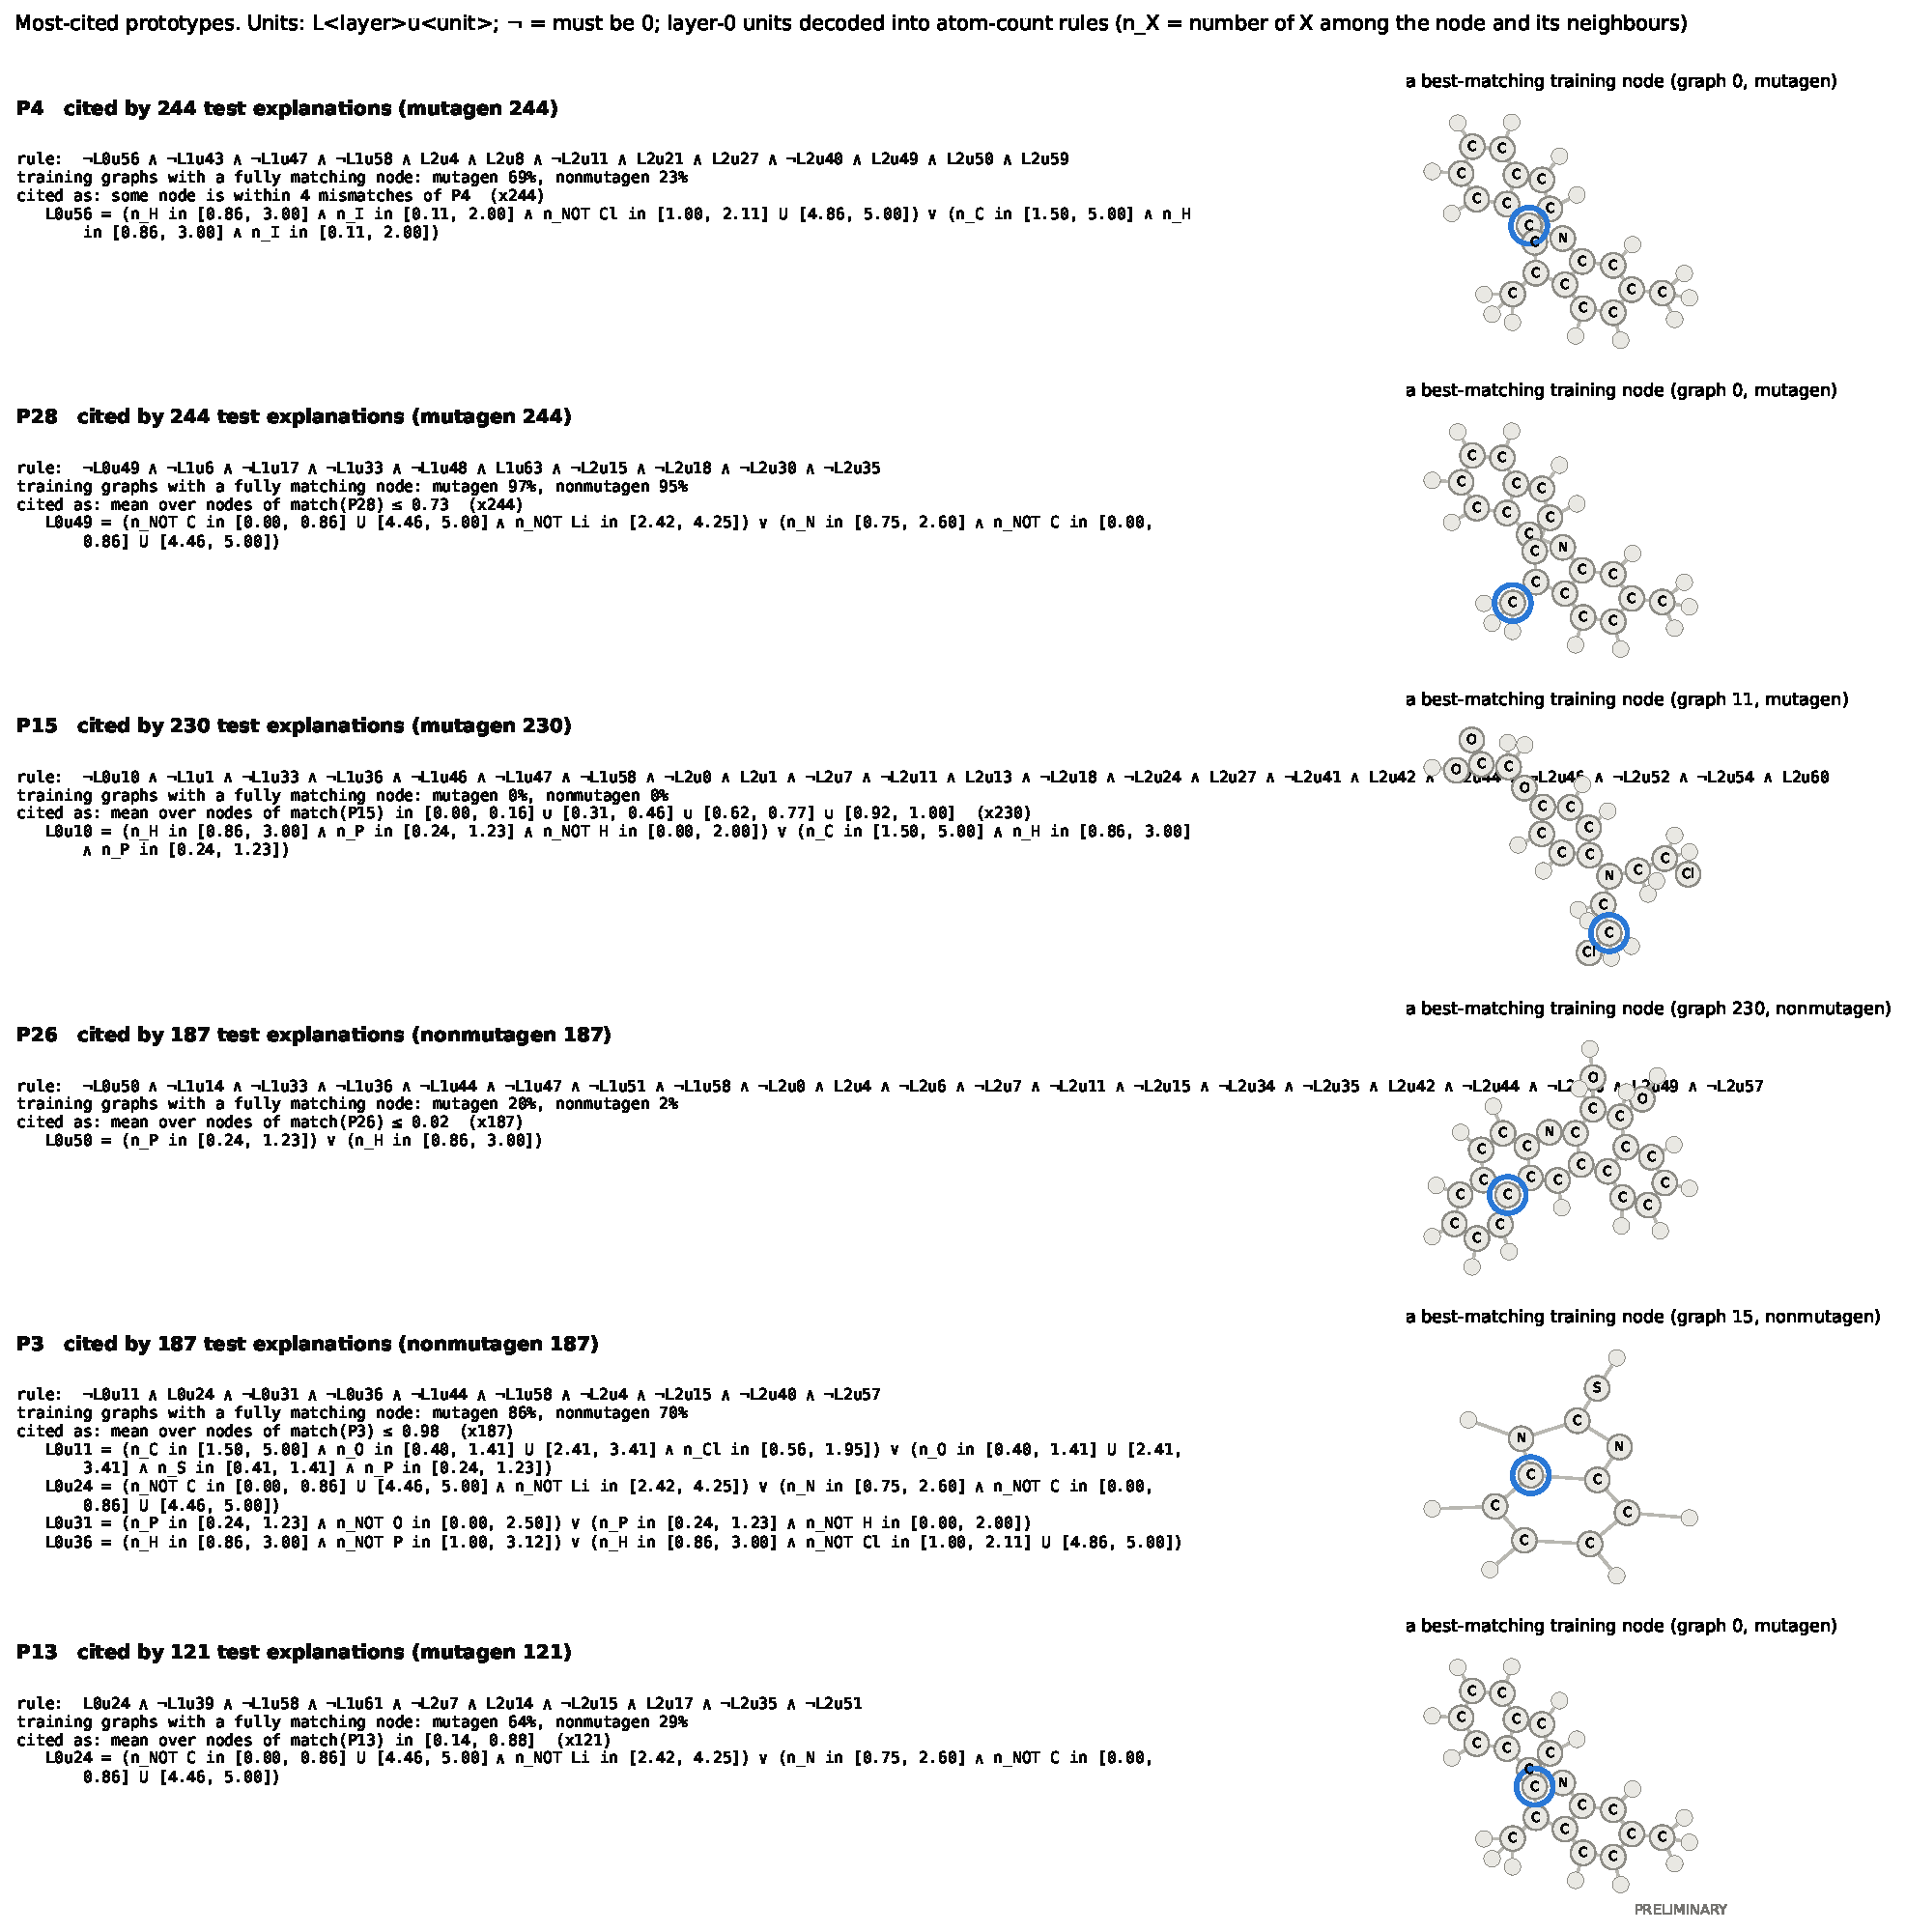
\includegraphics[width=\textwidth]{figures/fig_prototypes_Mutagenicity.pdf}%
  }{\fbox{\parbox[c][3cm]{0.95\textwidth}{\centering\todo{fig\_prototypes\_Mutagenicity.pdf}}}}\\[4pt]
  \IfFileExists{figures/fig_prototypes_BaMultiShapes.pdf}{%
    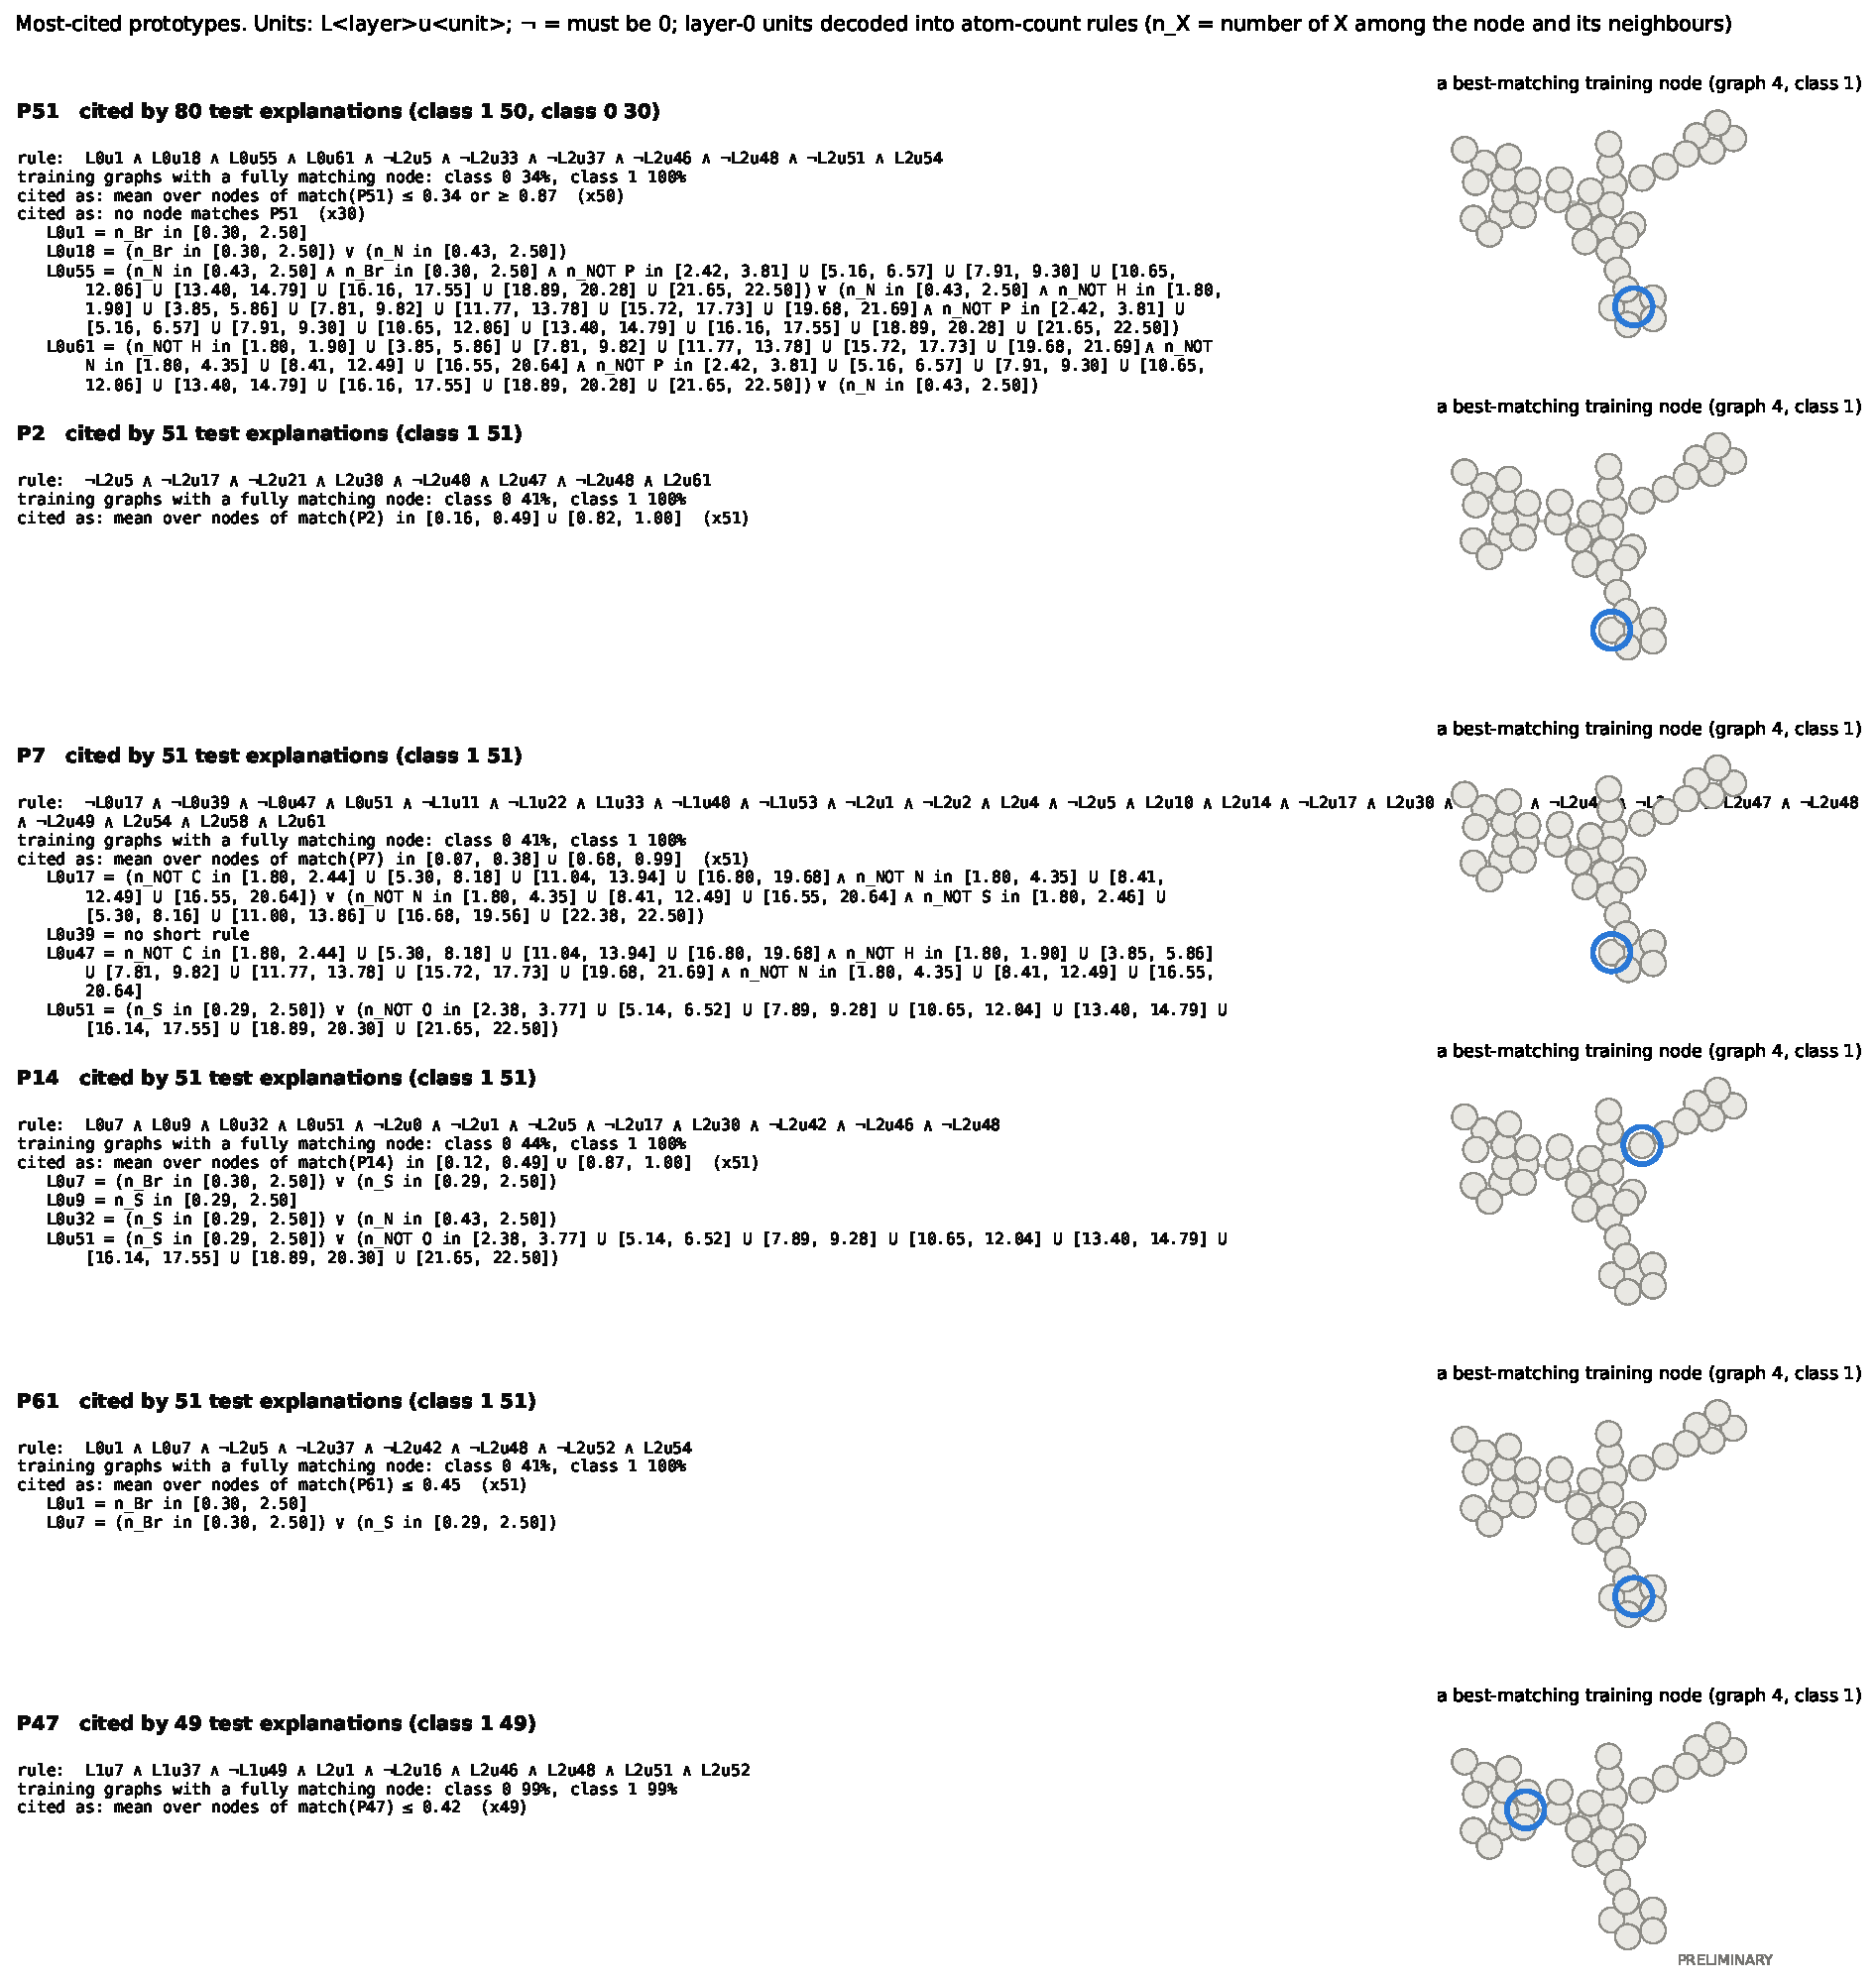
\includegraphics[width=\textwidth]{figures/fig_prototypes_BaMultiShapes.pdf}%
  }{\fbox{\parbox[c][3cm]{0.95\textwidth}{\centering\todo{fig\_prototypes\_BaMultiShapes.pdf}}}}\\[4pt]
  \caption{Prototypes of \oursqat{}. Each card shows the training node the
    prototype was projected on, the trunk conditions it cares about, and the best
    matching nodes of test graphs (highlighted; shaded: ground-truth region,
    NO$_2$/NH$_2$ on Mutagenicity, planted motifs on BAMultiShapes).}
  \label{fig:prototypes}
\end{figure*}
